\section{aggiungiContatto(ContattoRequest request)}

Il metodo  \colorbox{lightgray}{aggiungiContatto()}, appartenente alla classe DatiImpiegatoService, è responsabile dell’aggiunta di un contatto di riferimento per un agente immobiliare.
Per la verifica del suo corretto funzionamento è stata adottata una \textbf{strategia di testing white-box}, poiché il metodo presenta diversi flussi di controllo interni. Questa scelta consente di verificare che, a fronte di specifici input, il metodo segua il percorso logico previsto.
\\
In particolare, il metodo deve distinguere tra due casi:
\begin{enumerate}
	\item \textbf{Il contatto esiste già}: in questo scenario, il metodo aggiorna il valore del contatto esistente.
	\item \textbf{Il contatto non esiste}: in tal caso, viene aggiunto un nuovo elemento alla lista dei contatti.
\end{enumerate}
Di seguito è riportato il \textbf{grafo del flusso di controllo (GFC)}, utilizzato per rappresentare visivamente le diverse diramazioni logiche del metodo.

\begin{figure}[H]
	\centering
	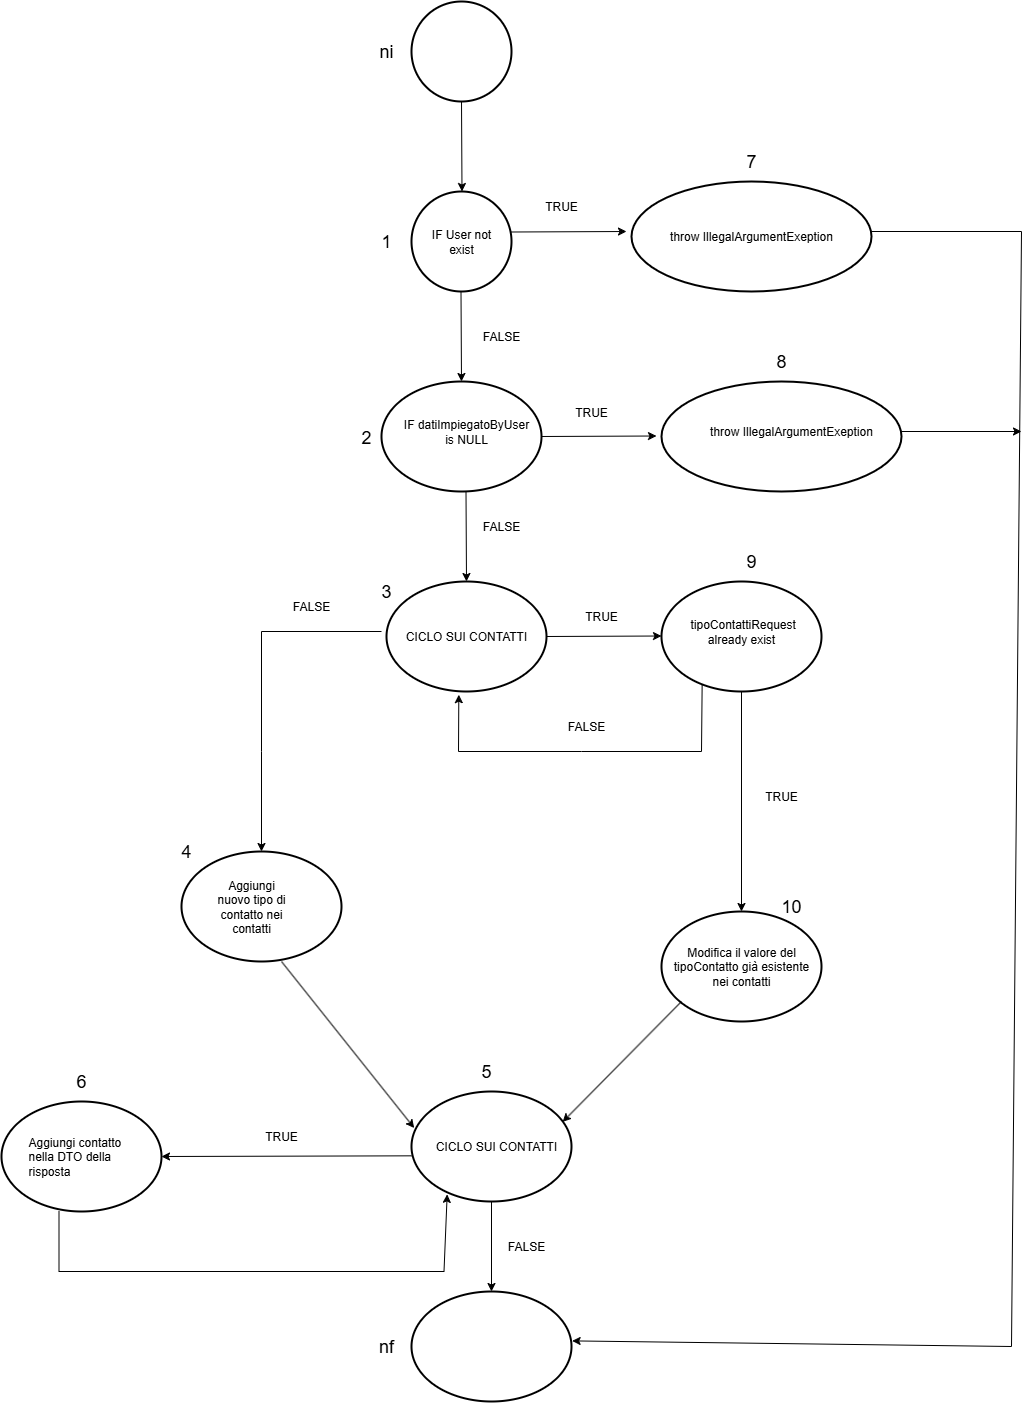
\includegraphics[width=0.7\linewidth]{Immagini/unit test/GrafoAggiungiUnContatto.png}
	\caption[GFC aggiungiContatto]{GFC del metodo aggiungiContatto(ContattoRequest request)}
\end{figure}

% Configurazione listings
\lstset{
	language=Java,                % Linguaggio di esempio
	backgroundcolor=\color{bgcolor}, % Colore di sfondo
	basicstyle=\ttfamily\small,     % Font e dimensione
	keywordstyle=\color{keywordcolor}\bfseries,
	commentstyle=\color{commentcolor}\itshape,
	stringstyle=\color{stringcolor},
	numbers=left,                   % Numeri a sinistra
	numberstyle=\tiny\color{gray},  % Stile dei numeri
	stepnumber=1,                   % Numeri in ogni riga
	numbersep=5pt,                  % Distanza dai numeri
	frame=single,                   % Cornice intorno al codice
	rulecolor=\color{gray},         % Colore della cornice
	tabsize=4,                       % Tab = 4 spazi
	showstringspaces=false,
	breaklines=true,                  % A capo automatico se troppo lungo
	literate=
	{à}{{\`a}}1
	{è}{{\`e}}1
	{é}{{\'e}}1
	{ì}{{\`i}}1
	{ò}{{\`o}}1
	{ù}{{\`u}}1
}


I test eseguiti hanno lo scopo di testare tutti i cammini possibili del grafo.

\begin{lstlisting}
	/**
	* Test verifica l'eccezione in caso di UserCurrent non trovato.
	* Copertura 1-7
	*/
	@Test
	void aggiungiContatto_ShouldThrowUnauthorizedException_
		WhenUserContextNotFound(){
		
			mocked.when(UserContex::getUserCurrent).thenReturn(null);
			
			assertThrows(it.unina.dietiestates25.exception.UnauthorizedException.class, () ->
			datiImpiegatoService.aggiungiContatto(request));
	}
\end{lstlisting}

\begin{lstlisting}
		/**
		* verifica che venga lanciata una ResourceNotFoundException quando l'utente non viene trovato nel database.
		* Copertura cammino 1-2-8
		*/
		@Test
		void aggiungiContatto_ShouldThrowResourceNotFoundException_
			WhenUserNotFoundInDB(){
			
				User mockUser = new User();
				
				mocked.when(UserContex::getUserCurrent).thenReturn(mockUser);
				when(datiImpiegatoRepository.findDatiImpiegatoByUser(mockUser)).thenReturn(Optional.empty());
				
				assertThrows(it.unina.dietiestates25.exception.ResourceNotFoundException.class, () ->
				datiImpiegatoService.aggiungiContatto(request));
			
		}
\end{lstlisting}

\begin{lstlisting}
	 /**
	* Verifica che aggiunge un nuovo contatto tra i contatti già esistenti dell'agente
	* Copertura cammino 1-2-3-4-5-6-5
	*/
	@Test
	void aggiungiContatto_
	ShouldAddNewContactWithoutExistingContacts(){
		
			request.setTipo("Cellulare");
			request.setValore("338469123");
			
			List<ContattoResponse> response = datiImpiegatoService.aggiungiContatto(request);
			
			//Controlli sul nuovo stato dei contatti esistenti dell'agente
			assertTrue(contattiEsistenti.size() == 1);
			assertTrue(contattiEsistenti.get(0).getTipo().equals("Cellulare"));
			assertTrue(contattiEsistenti.get(0).getValore().equals("338469123"));
			
			//Controlli sulla DTO in risposta
			assertTrue(response.size() == 1);
			
			assertTrue(response.get(0).getTipo().equals("Cellulare"));
			assertTrue(response.get(0).getValore().equals("338469123"));
	}
\end{lstlisting}

\begin{lstlisting}
	/**
	* Verica che aggiunge un nuovo contatto (come sopra ma con almeno un iterazione tra i contati esistenti)
	*Copertura cammino 1-2-3-9-3-4-5-6-5-6-5
	*/
	@Test
	void aggiungiContatto_
	ShouldAddNewConcatWithExistingContacts(){
		
			Contatto contatto = Contatto.builder()
			.tipo("Cellulare")
			.valore("3338469123")
			.build();
			
			contattiEsistenti.add(contatto);
			
			request.setTipo("Email");
			request.setValore("roby@gmail.com");
			
			List<ContattoResponse> response = datiImpiegatoService.aggiungiContatto(request);
			
			//Controlli sul nuovo stato dei contatti esistenti dell'agente
			assertTrue(contattiEsistenti.size() == 2);
			
			assertTrue(contattiEsistenti.get(0).getTipo().equals("Cellulare"));
			assertTrue(contattiEsistenti.get(0).getValore().equals("3338469123"));
			
			assertTrue(contattiEsistenti.get(1).getTipo().equals("Email"));
			assertTrue(contattiEsistenti.get(1).getValore().equals("roby@gmail.com"));
			
			//Controlli sulla DTO in risposta
			assertTrue(response.size() == 2);
			
			assertTrue(response.get(0).getTipo().equals("Cellulare"));
			assertTrue(response.get(0).getValore().equals("3338469123"));
			
			assertTrue(response.get(1).getTipo().equals("Email"));
			assertTrue(response.get(1).getValore().equals("roby@gmail.com"));
	}
\end{lstlisting}

\begin{lstlisting}
	/**
	* verifica che si accorge che il contatto è un tipo già esistente e quindi deve modificarne il valore non aggiungere uno nuovo.
	* Copertura cammino 1-2-3-9-3-9-10-5-6-5-6-5
	*/
	@Test
	void aggiungiContatto_ShouldModifyExistingContact(){
		
		Contatto contatto1 = Contatto.builder()
		.tipo("Cellulare")
		.valore("3338469123")
		.build();
		
		Contatto contatto2 = Contatto.builder()
		.valore("roby@gmail.com")
		.tipo("Email")
		.build();
		
		contattiEsistenti.add(contatto1);
		contattiEsistenti.add(contatto2);
		
		request.setTipo("Email");
		request.setValore("raimondo@gmail.com");
		
		List<ContattoResponse> response = datiImpiegatoService.aggiungiContatto(request);
		
		//Controlli sul nuovo stato dei contatti esistenti dell'agente
		assertTrue(contattiEsistenti.size() == 2);
		
		assertTrue(contattiEsistenti.get(0).getTipo().equals("Cellulare"));
		assertTrue(contattiEsistenti.get(0).getValore().equals("3338469123"));
		
		assertTrue(contattiEsistenti.get(1).getTipo().equals("Email"));
		assertTrue(contattiEsistenti.get(1).getValore().equals("raimondo@gmail.com"));
		
		//Controlli sulla DTO in risposta
		assertTrue(response.size() == 2);
		
		assertTrue(response.get(0).getTipo().equals("Cellulare"));
		assertTrue(response.get(0).getValore().equals("3338469123"));
		
		assertTrue(response.get(1).getTipo().equals("Email"));
		assertTrue(response.get(1).getValore().equals("raimondo@gmail.com"));
		
	}
\end{lstlisting}

\begin{lstlisting}
	  /**
	* verifica che si accorge di moficare il valore di un contatto invece di aggiungerlo uno nuovo. (Stessa verifica di sopra ma senza iterazione nel ciclo)
	* Copertura cammino 1-2-3-9-10-5-6-5
	*/
	@Test
	void aggiungiContatto_
	ShouldModifyExistingContactWithoutIteration(){
		
			Contatto contatto = Contatto.builder()
			.tipo("Cellulare")
			.valore("3338469123")
			.build();
			
			contattiEsistenti.add(contatto);
			
			request.setTipo("Cellulare");
			request.setValore("31520289137");
			
			List<ContattoResponse> response = datiImpiegatoService.aggiungiContatto(request);
			
			//Controlli sul nuovo stato dei contatti esistenti dell'agente
			assertTrue(contattiEsistenti.size() == 1);
			
			assertTrue(contattiEsistenti.get(0).getTipo().equals("Cellulare"));
			assertTrue(contattiEsistenti.get(0).getValore().equals("31520289137"));
			
			//Controlli sulla DTO in risposta
			assertTrue(response.size() == 1);
			
			assertTrue(response.get(0).getTipo().equals("Cellulare"));
			assertTrue(response.get(0).getValore().equals("31520289137"));
		
	}
\end{lstlisting}

\begin{figure}[H]
	\centering
	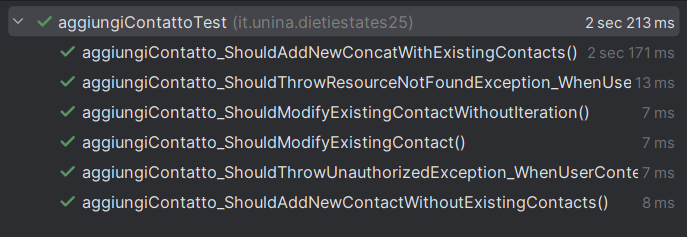
\includegraphics[width=0.7\linewidth]{Immagini/unit test/esitiTestaddContatto.png}
	\caption[Esito test 3]{Screen che riporta l'esito positivo dei test}
\end{figure}
